\chapter{Experiments}\label{sec:experiments}

%The task of the \glspl{nn} is to classify each flow into either \textit{benign} or \textit{attack} which results in a binary classification problem. Ordinary network traffic that should be ignored by the \gls{ids} is labeled as \textit{benign} and flows that constitute or are part of a cyber-attack are labeled as \textit{attack}. As there are only two possible labels, \gls{bce} can be used as loss function to determine the distance between the predicted label by the \glspl{nn} and the actual label \todo{give more detailed explaination of BCE Loss}. 

As a premise for our research we trained the \gls{lstm} and the transformer network in a solely supervised fashion to get a baseline later results can be compared to. Supervised training was performed for 50, 200 and 600 epochs each for 90\%, 10\% and 1\% respectively of available data on both data-sets and a constant 10\% of data for validation which has not been used for training. A full overview of all experiments to establish a comparison baseline can be seen in \ref{table:experiments:baseline}. We specifically wanted to know how the networks would perform in a scenario where very little labeled training data was available as this would best describe a scenario where large amounts of unlabeled data are available for self-supervised pre-training and only a small amount of labeled data for fine tuning. To pre-train a \gls{nn} the network is given a task that is not necessarily connected to the final purpose of the network, often referred to as a \textit{proxy task}. By solving the proxy task the network attempts to find structure in the data and should learn to form a more abstract representation of the data within its latent space. E.g. with \gls{bert} pre-training is performed by masking a certain percentage of input tokens and having the \gls{nn} reconstruct the missing words and additionally letting the network guess whether one sentences precedes another in a text. We defined our own proxy tasks for pre-training the networks as described in the following sections. Pre-training is performed with 80\% of available data, supervised fine-tuning with 10\%, 1\% and with even smaller subsets as described in the previous section \ref{sec:methodology:subsets}. \par
The idea behind these experiments is to reduce the available labeled data to highlight positive effects resulting from pre-training. The assumption is: The less the model can rely on information acquired through supervised training the more it has to rely on information acquired during self-supervised pre-training. Overviews of all conducted experiments can be found in tables \ref{table:experiments:baseline}, \ref{table:experiments:lstm:configurations} and \ref{table:experiments:transformer:configurations}.
Experiments are numbered so they can be referenced in later sections. Experiments in table \ref{table:experiments:baseline} where the model is not pre-trained are referenced again in table \ref{table:experiments:lstm:configurations}.

\begin{table}[h]
	\scalebox{0.92}{
		\begin{tabular}{c c c c c c c}
			\textbf{\#} & \textbf{Model} & \textbf{Dataset} & \multicolumn{1}{l}{\textbf{Batch size}} & \textbf{Subset} & \textbf{Training \%} & \multicolumn{1}{l}{\textbf{Training Eps.}} \\ \hline \midrule
			1.1.1 \label{ex_1_1_1}           & LSTM           & CIC-IDS2017     & 128                                     & - 		& 90                   & 50                                            \\ \midrule
			2.1.1 \label{ex_1_1_2}           & LSTM           & CIC-IDS2017     & 128                                     & - 		& 10                   & 50                                            \\ \midrule
			2.2.1 \label{ex_1_1_3}           & LSTM           & CIC-IDS2017     & 128                                     & - 		& 1                    & 200                                           \\ \midrule
			2.3.1 \label{ex_1_1_4}           & LSTM           & CIC-IDS2017     & 128                                     & CIC17\_10	& -                    & 600                                           \\ \midrule
			1.2.1 \label{ex_1_1_5}           & LSTM           & UNSW-NB15        & 128                                     & -			& 90                   & 50                                            \\ \midrule
			2.4.1 \label{ex_1_1_6}           & LSTM           & UNSW-NB15        & 128                                     & -			& 10                   & 50                                            \\ \midrule
			2.5.1 \label{ex_1_1_7}           & LSTM           & UNSW-NB15        & 128                                     & -			& 1                    & 200                                           \\ \midrule
			2.6.1 \label{ex_1_1_8}           & LSTM           & UNSW-NB15        & 128                                     & CIC17\_10	& -                    & 600                                           \\ \midrule
			1.3.1 \label{ex_1_2_1}           & transformer    & CIC-IDS2017     & 1024                                     & -			& 90                   & 50                                            \\ \midrule
			3.1.1 \label{ex_1_2_2}           & transformer    & CIC-IDS2017     & 1024                                     & -			& 10                   & 50                                            \\ \midrule
			3.2.1 \label{ex_1_2_3}           & transformer    & CIC-IDS2017     & 1024                                     & -			& 1                    & 200                                           \\ \midrule
			3.3.1 \label{ex_1_2_4}           & transformer    & CIC-IDS2017     & 1024                                     & UNSW15\_10	& -                    & 600                                           \\ \midrule
			1.4.1 \label{ex_1_2_5}           & transformer    & UNSW-NB15        & 1024                                     & -			& 90                   & 50                                            \\ \midrule
			3.4.1 \label{ex_1_2_6}           & transformer    & UNSW-NB15        & 1024                                     & -			& 10                   & 50                                            \\ \midrule
			3.5.1 \label{ex_1_2_7}           & transformer    & UNSW-NB15        & 1024                                     & -			& 1                    & 200                                           \\ \midrule
			1.6.1 \label{ex_1_2_8}           & transformer    & UNSW-NB15        & 1024                                     & UNSW15\_10	& -                    & 600                                           \\
	\end{tabular}}
	\caption{List of baseline training runs used for comparison later in the thesis.}
	\label{table:experiments:baseline}
\end{table}

As pre-training method we devised a list of proxy tasks which should challenge the model to build an abstract representation of the data within its hidden space or at least learn which features are more important than others and correct weights accordingly. A list of all proxy tasks can be seen in table \ref{table:experiments:proxy_tasks}. Each of them will be explained in detail in the sections below.

\begin{table}[H]
	\centering
	\begin{tabular}{c c c c}
		\thead{\textbf{Section(s)}} & \thead{\textbf{Label}} & \thead{\textbf{Name}} & \thead{\textbf{Description}} \\ \hline \midrule
		\ref{sec:experiments:lstm:identity} & IDENTITY & Identity Function & \makecell{Reconstruct exact input \\ feature vector at each stage} \\ \midrule
		\ref{sec:experiments:lstm:predict_packet} & PREDICT & Predict Packet & \makecell{Predict the next packet at \\ each stage of the \gls{lstm}} \\ \midrule
		\ref{sec:experiments:lstm:mask_packet}, \ref{sec:experiments:transformer:mask_packet} & MASK & Mask Packets & \makecell{Reconstruct masked packets \\ in the sequence} \\ \midrule
		\ref{sec:experiments:lstm:obscure}, \ref{sec:experiments:transformer:mask_feature} & OBSCURE & Obscure Features & \makecell{Reconstruct obscured features} \\ \midrule
		\ref{sec:experiments:lstm:auto_encoder}, \ref{sec:experiments:transformer:auto_encoder} & AUTO & Auto-Encoder & \makecell{Encode and decode input \\ with minimal loss} \\ \midrule\\
		\ref{sec:experiments:lstm:composite} & COMPOSITE & Composite Task & \makecell{Combination of prediction \\ and auto-encoding} \\ \midrule\\
	\end{tabular}
	\caption{Devised proxy tasks for pre-training of \gls{dl} models.}
	\label{table:experiments:proxy_tasks}
\end{table}

\section{Self-supervised Pre-training for Long Short-Term Memory Networks} \label{sec:experiments:lstm}

For pre-training the \gls{lstm} we devised six different proxy tasks for the model to solve in a self-supervised fashion: Predicting the next packet in the flow, predicting masked features of randomly chosen packets and predicting randomly masked packets, the identity function, a sequence2sequence auto-encoder and a composite task comprised of part auto encoding and part prediction. 
The weights of each \gls{lstm} layer are initialized with a uniform random distribution $\mathcal{U}(-\sqrt{k}, \sqrt{k})$ where $k = \frac{1}{\text{hidden\_size}}$. Because we assume that in some cases, i.e. for some sequences, no reasonable prediction can be made we don't want the model to react too strongly to those outliers. Hence, the \gls{mae} is used to determine the divergence between prediction and target data instead of \gls{mse}. Translating to PyTorch this means we used \textit{L1Loss} with \textit{mean} reduction as the loss function for pre-training. After some initial trials we set the training hyper-parameters for both supervised and self-supervised training to an initial \textit{learning rate} of $10^{-3}$ and a \textit{batch size} of 128. Over the training process, the learning rate will be adjusted by Adam so the model is somewhat robust to changes on the initial learning rate. For every proxy task, the model has been trained with the different parameters in table \ref{table:experiments:lstm:configurations} to establish comparable results.

\begin{table}[h]
	\scalebox{0.8}{
	\begin{tabular}{cccccccc}
		\textbf{\#}    & \textbf{Dataset}      & \textbf{Subset}     & \textbf{Training} \% & \textbf{Training Eps.} & \textbf{Proxy Task} & \textbf{Pretr.} \% & \textbf{Pretr. Eps.} \\ \hline
		2.1.1 \label{ex_2_1_1} & CIC-IDS2017 & -          & 10          & 50            & NONE       & 0         & 0           \\
		2.1.2 \label{ex_2_1_2} & CIC-IDS2017 & -          & 10          & 50            & PREDICT    & 80        & 10          \\
		2.1.3 \label{ex_2_1_3} & CIC-IDS2017 & -          & 10          & 50            & OBSCURE      & 80        & 10          \\
		2.1.4 \label{ex_2_1_4} & CIC-IDS2017 & -          & 10          & 50            & AUTO       & 80        & 10          \\
		2.1.5 \label{ex_2_1_5} & CIC-IDS2017 & -          & 10          & 50            & IDENTITY   & 80        & 10          \\
		2.1.6 \label{ex_2_1_6} & CIC-IDS2017 & -          & 10          & 50            & COMPOSITE  & 80        & 10          \\
		2.2.1 \label{ex_2_2_1} & CIC-IDS2017 & -          & 1           & 200           & NONE       & 0         & 0           \\
		2.2.2 \label{ex_2_2_2} & CIC-IDS2017 & -          & 1           & 200           & PREDICT    & 80        & 10          \\
		2.2.3 \label{ex_2_2_3} & CIC-IDS2017 & -          & 1           & 200           & OBSCURE      & 80        & 10          \\
		2.2.4 \label{ex_2_2_4} & CIC-IDS2017 & -          & 1           & 200           & AUTO       & 80        & 10          \\
		2.2.5 \label{ex_2_2_5} & CIC-IDS2017 & -          & 1           & 200           & IDENTITY   & 80        & 10          \\
		2.2.6 \label{ex_2_2_6} & CIC-IDS2017 & -          & 1           & 200           & COMPOSITE  & 80        & 10          \\
		2.3.1 \label{ex_2_3_1} & CIC-IDS2017 & CIC17\_10  & -           & 600           & NONE       & 0         & 0           \\
		2.3.2 \label{ex_2_3_2} & CIC-IDS2017 & CIC17\_10  & -           & 600           & PREDICT    & 80        & 10          \\
		2.3.3 \label{ex_2_3_3} & CIC-IDS2017 & CIC17\_10  & -           & 600           & OBSCURE      & 80        & 10          \\
		2.3.4 \label{ex_2_3_4} & CIC-IDS2017 & CIC17\_10  & -           & 600           & AUTO       & 80        & 10          \\
		2.3.5 \label{ex_2_3_5} & CIC-IDS2017 & CIC17\_10  & -           & 600           & IDENTITY   & 80        & 10          \\
		2.3.6 \label{ex_2_3_6} & CIC-IDS2017 & CIC17\_10  & -           & 600           & COMPOSITE  & 80        & 10          \\
		2.4.1 \label{ex_2_4_1} & UNSW-NB15    & -          & 10          & 50            & NONE       & 0         & 0           \\
		2.4.2 \label{ex_2_4_2} & UNSW-NB15    & -          & 10          & 50            & PREDICT    & 80        & 10          \\
		2.4.3 \label{ex_2_4_3} & UNSW-NB15    & -          & 10          & 50            & OBSCURE      & 80        & 10          \\
		2.4.5 \label{ex_2_4_4} & UNSW-NB15    & -          & 10          & 50            & AUTO       & 80        & 10          \\
		2.4.6 \label{ex_2_4_5} & UNSW-NB15    & -          & 10          & 50            & IDENTITY   & 80        & 10          \\
		2.4.7 \label{ex_2_4_6} & UNSW-NB15    & -          & 10          & 50            & COMPOSITE  & 80        & 10          \\
		2.5.1 \label{ex_2_5_1} & UNSW-NB15    & -          & 1           & 200           & NONE       & 0         & 0           \\
		2.5.2 \label{ex_2_5_2} & UNSW-NB15    & -          & 1           & 200           & PREDICT    & 80        & 10          \\
		2.5.3 \label{ex_2_5_3} & UNSW-NB15    & -          & 1           & 200           & OBSCURE      & 80        & 10          \\
		2.5.4 \label{ex_2_5_4} & UNSW-NB15    & -          & 1           & 200           & AUTO       & 80        & 10          \\
		2.5.5 \label{ex_2_5_5} & UNSW-NB15    & -          & 1           & 200           & IDENTITY   & 80        & 10          \\
		2.5.6 \label{ex_2_5_6} & UNSW-NB15    & -          & 1           & 200           & COMPOSITE  & 80        & 10          \\
		2.6.1 \label{ex_2_6_1} & UNSW-NB15    & UNSW15\_10 & -           & 600           & NONE       & 0         & 0           \\
		2.6.2 \label{ex_2_6_2} & UNSW-NB15    & UNSW15\_10 & -           & 600           & PREDICT    & 80        & 10          \\
		2.6.3 \label{ex_2_6_3} & UNSW-NB15    & UNSW15\_10 & -           & 600           & OBSCURE      & 80        & 10          \\
		2.6.4 \label{ex_2_6_4} & UNSW-NB15    & UNSW15\_10 & -           & 600           & AUTO       & 80        & 10          \\
		2.6.5 \label{ex_2_6_5} & UNSW-NB15    & UNSW15\_10 & -           & 600           & IDENTITY   & 80        & 10          \\
		2.6.6 \label{ex_2_6_6} & UNSW-NB15    & UNSW15\_10 & -           & 600           & COMPOSITE  & 80        & 10         
	\end{tabular}}
	\caption{Training and pre-training configurations for \gls{lstm} model with different proxy tasks.}
	\label{table:experiments:lstm:configurations}
\end{table}

\subsection{Identity Function (IDENTITY)} \label{sec:experiments:lstm:identity}

The simplest form of a proxy-task for pre-training is having the model learn the identity function. In practice this means that input sequence $x^{(t)}$ and target sequence $y^{(t)}$ are the same i.e. $x^{(t)} = y^{(t)}$ with the same sequence length. The model learns to convey the information through the network at each time step. For this task, the model does not need to derive any meaningful hidden representation of the data, but as our experiments show it still moves the weights of the model into a favorable direction in some instances when compared to the case where the model was not pre-trained, i.e. where weights are initialized randomly with a uniform distribution.

\begin{figure}[h]
	\centering
	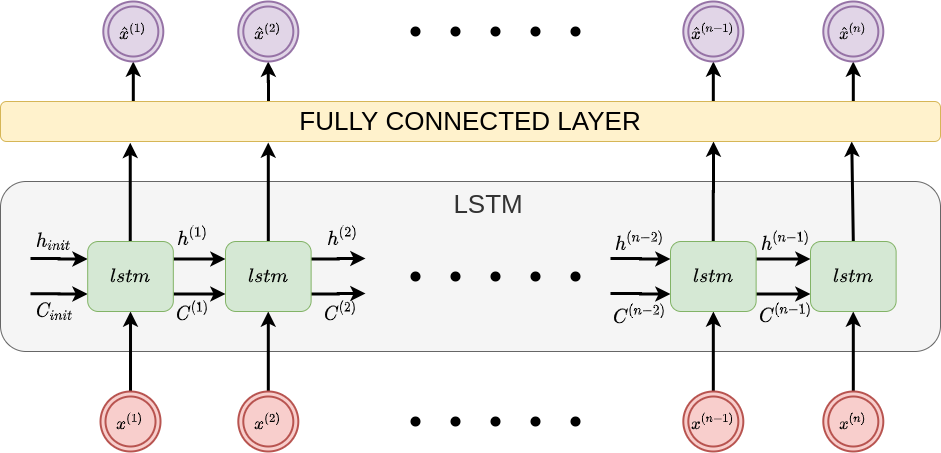
\includegraphics[width=1.0\textwidth]{img/lstm_proxy_task_id.png}
	\caption{Depiction of data flow, input and output of the model during pre-training on the identity function proxy task (ID).}
	\label{fig:experiments:lstm_proxy_task_id}
\end{figure}

\subsection{Predict Packet (PREDICT)} \label{sec:experiments:lstm:predict_packet}

For this proxy task, the model has to predict the next packet in the flow. We started by predicting only the last packet in each flow but then moved to predicting all packets in a flow except the first. This means having a \textit{sequence-to-sequence} model where the inputs are all tokens in one flow with length $n$ except the last, because it has no successor: $x^{(t)} = x^{(1)}, x^{(2)}, ..., x^{(n-1)}$. The target data are all tokens in the same flow except the first, because it has no predecessor: $y^{(t)} = x^{(t+1)} : t = 1,..,n-1$. \glspl{lstm} process data in sequential order so at each time step, the model only has information of packets in the past and is to predict what the next packet in the flow will be. This results in two comparable tensors $y^{(t)}$ and the model output sequence $\hat{y}^{(t)} = \hat{y}^{(1)}, \hat{y}^{(2)}, ..., \hat{y}^{(n-1)}$ of equal length $n-1$ between which a differentiable loss can be calculated. This way, a lot of information is conveyed to the network when compared to only predicting the last packet in a flow. At first glance, this looks similar to the identity function in \ref{sec:experiments_lstm_identity}. The key difference however, is that the token which is to be predicted is not yet available as an input token to the model, meaning it has to derive the features by other means than conveying the requested input token to the output. The loss is calculated as the \gls{mae} (\textit{L1Loss} with \textit{mean} reduction) between the predicted logits and the target data sequences.

\begin{figure}[h]
	\centering
	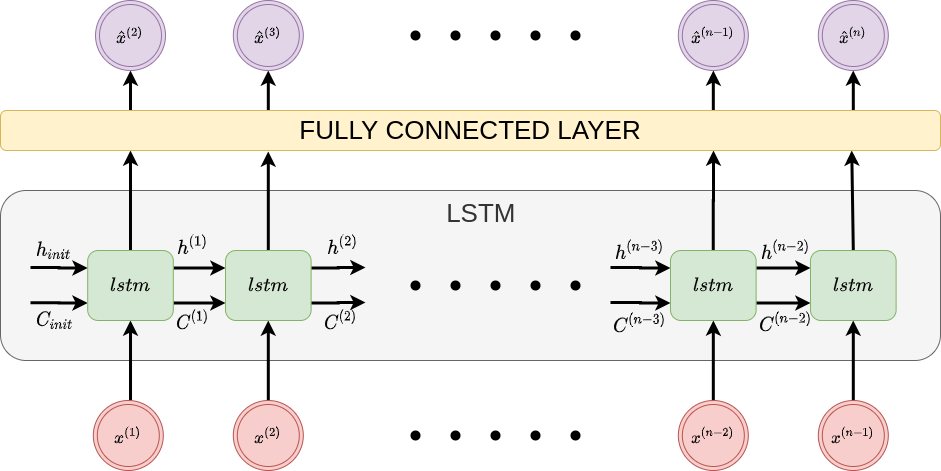
\includegraphics[width=1.0\textwidth]{img/lstm_proxy_task_predict.png}
	\caption{Depiction of data flow, input and output of the model during pre-training on the prediction proxy task (PREDICT).}
	\label{fig:experiments:lstm_proxy_task_predict}
\end{figure}

\subsection{Mask Packets (MASK)} \label{sec:experiments:lstm:mask_packet}

Similar to the pre-training in \gls{bert}, all features of a random packet in the sequence is masked with a value of -1, i.e. the token is replaced with a feature vector $x_{mask} = [-1, ..., -1]^T$ containing $-1$ for each element and the model is to predict the masked token. Again, \gls{mae} is used as the loss function. Unlike to \gls{bert}, we don't only look at the masked tokens when calculating the loss but compare every feature of every packet, also the non-masked ones, which adds an auto-encoding property to the pre-training. We found this to have more beneficial effect on the results than only looking at the masked packets. This is possibly due to the model having to retain information to solve two different tasks, an approach also used by to pre-train Google's BERT,  which prevents the model from attuning itself to one specific task by losing generality.

\begin{figure}[h]
	\centering
	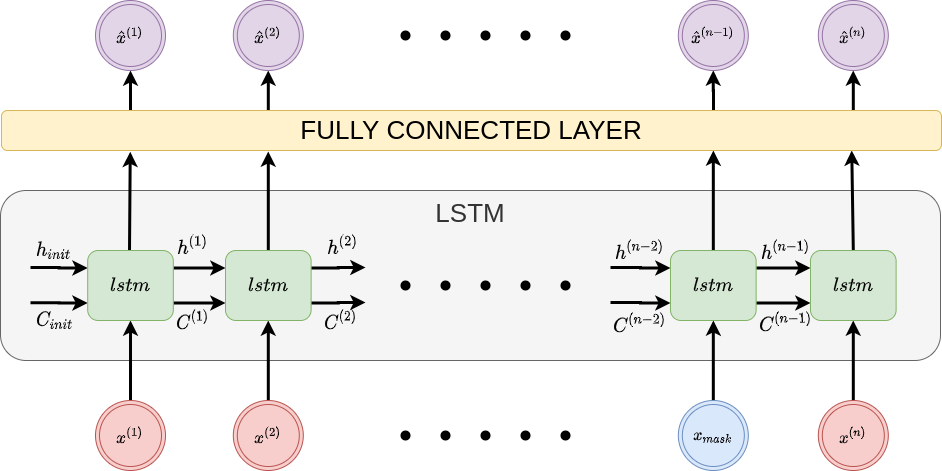
\includegraphics[width=1.0\textwidth]{img/lstm_proxy_task_mask.png}
	\caption{Depiction of data flow, input and output of the model during pre-training on the mask packet proxy task (MASK).}
	\label{fig:experiments:lstm_proxy_task_mask}
\end{figure}

\subsection{Obscure Features (OBSCURE)} \label{sec:experiments:lstm:obscure}

For this pre-training task, the model is to predict masked features of some packets in the sequence. We have tried multiple masking values but $-1$ produces the best results out of the values we tried. This proxy task in particular can be parameterized in different ways. E.g. the number of features and which features to mask, if always the same features are masked or if the selection is random for each packet or for each flow, if every packet in the sequence has some masked features or if there is only a chance that a packet is selected for masking. Those are only some examples of how this task can be set up in different ways. To be completely exhaustive was not possible, but we tried some of the most intuitive approaches. The task proved to be quite difficult for both models, so we decided to predict only the TCP SYN flag. For pre-training the model is provided masked data as input sequence and the unmasked data is the target. The loss is calculated as the \gls{mae} (\textit{L1Loss} with \textit{mean} reduction) between the obscured features of predicted \textit{logits} and the target data sequences.

\begin{figure}[h]
	\centering
	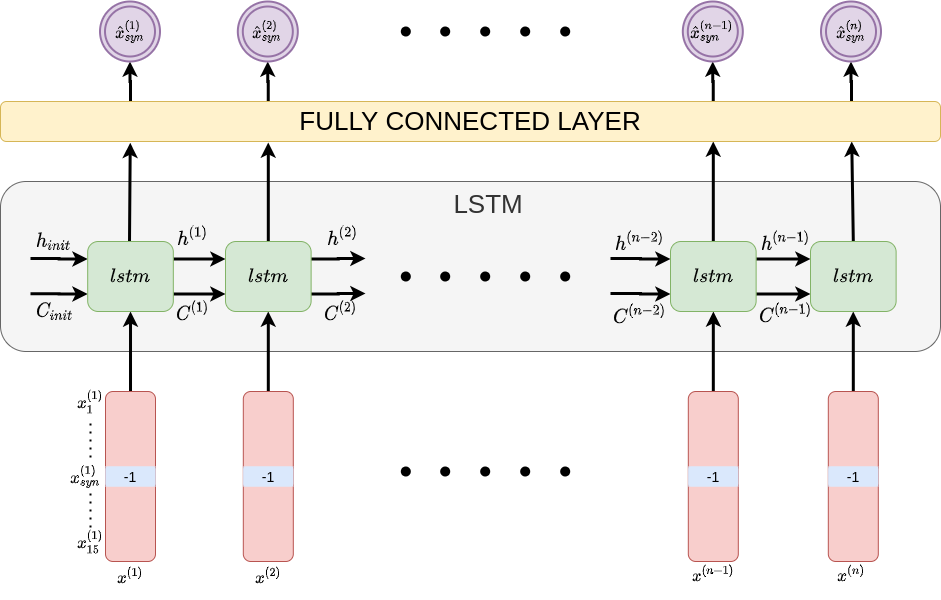
\includegraphics[width=1.0\textwidth]{img/lstm_proxy_task_obscure.png}
	\caption{Depiction of data flow, input and output of the model during pre-training on the obscure feature proxy task (OBSCURE).}
	\label{fig:experiments:lstm_proxy_task_obscure}
\end{figure}

\subsection{Auto Encoder (AUTO)} \label{sec:experiments:lstm:auto_encoder}

As explained in section \ref{sec:backgrund:autoencoder}, for the auto encoder the model is tasked with compressing and decompressing the data as lossless as possible. With an \gls{lstm} model, this means having two consecutive \gls{lstm} models where the first is to encode the sequence and the second is to decode the sequence. As template we used the model proposed by Nitish Srivastava et al. in their paper "Unsupervised Learning of Video Representations using LSTMs" \cite{unsupervised_learning_lstms}, but similar proposals for Auto-Encoders with \glspl{lstm} can be found in \cite{unsupervised_learning_lstms_timeseries} or \cite{lstm_anomaly_detection}. \par
The encoder \gls{lstm} compresses the whole input sequence $x_e^{(t)} = x_e^{(1)}, x_e^{(2)}, ..., x_e^{(n)}$ into the hidden state of the last stage $h_e^{(n)}$ ($C_e^{(n)}$) where $n$ is the length of the input sequence. The decoder \gls{lstm} is then initialized with the hidden and cell state of the last stage from the encoder \gls{lstm} $h_d^{(1)} = h_e^{(n)}, C_d^{(1)} = C_e^{(n)}$ and is tasked with reconstructing the input sequence in reverse order. The reverse order is used to shorten the paths of the initial target tokens to their respecting input tokens. After every stage of the decoder, either the output of the current stage $\hat{y}^{(t)}$ or the target token of the current stage $x^{(t)}$, the ground truth, is then fed into the model as input token $x_d^{(t+1)} = \hat{x}^{(t)}$ for the next stage. The first method is also called \textit{autoregression}. The first input token for the decoder is a zero vector which functions as a start-of-sequence token $x_{zero} = [0, ..., 0]^T$. This way, the encoder is forced to store as much information about the sequence as possible in the hidden state and as the size of the hidden state is constrained, it has to find an abstract representation of the sequence. For supervised fine-tuning and validation, only the encoder part of the model is used. After trying both approaches, we decided to use teacher forcing as it produced slightly better results.

\begin{figure}[h]
	\centering
	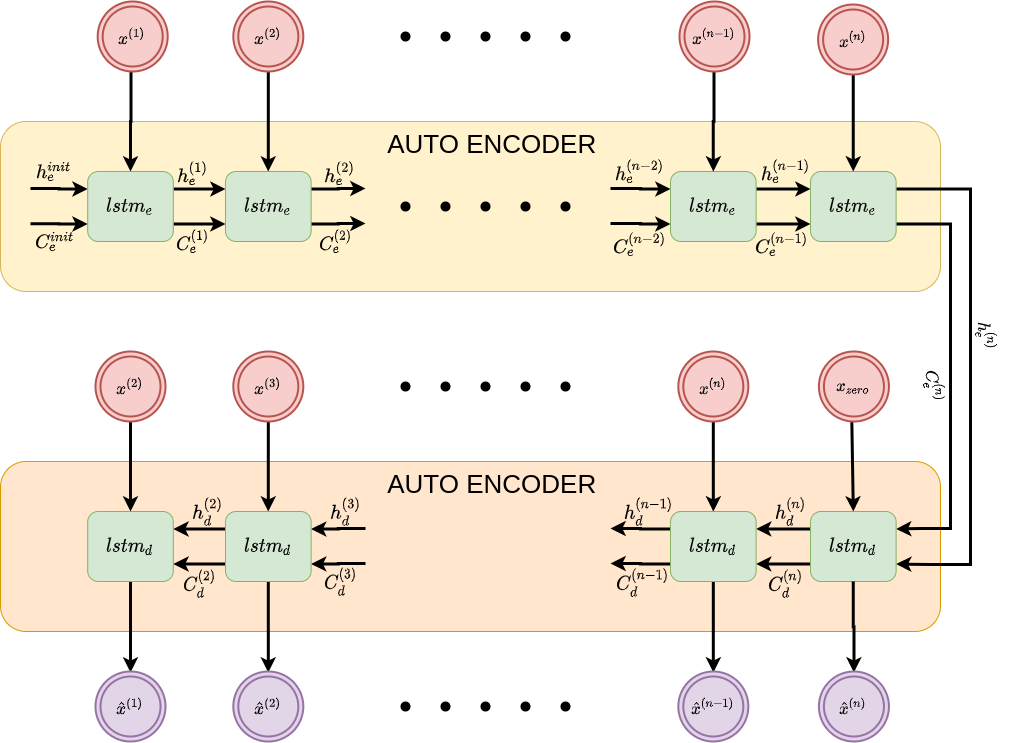
\includegraphics[width=1.0\textwidth]{img/lstm_proxy_task_auto.png}
	\caption{Depiction of data flow, input and output of the model during pre-training on auto encoder packet proxy task (AUTO).}
	\label{fig:experiments:lstm_proxy_task_auto}
\end{figure}

\subsection{Composite Model (COMPOSITE)} \label{sec:experiments:lstm:composite}

For the composite model we recreated the network proposed by Nitish Srivastava et al. in their paper "Unsupervised Learning of Video Representations using LSTMs" \cite{unsupervised_learning_lstms} as summarized in section \ref{sec:stateofart:unsupervised_video_lstm}. As a self-supervised pre-training proxy task, the model is fed half the packet sequence of a flow and is tasked with both reconstructing the part of the sequence it had access to, and predicting the missing part of the flow which it had no access to. The output of the model is a sequence $\hat{y}^{(t)}$ of length equal to the original input sequence $x^{(t)}$ of which the first half is reconstructed and the second half is predicted by the model. The loss is again calculated as the \gls{mae} (\textit{L1Loss} with \textit{mean} reduction) between the original input and the output sequence of the model. The model consists of three \glspl{lstm} which can be labeled \textit{encoder}, \textit{decoder} and \textit{predictor} as can be seen in figure \ref{fig:experiments:unsupervised_lstm_composite}. The encoder processes the first half of the original input sequence, constructing an abstract representation in its hidden state. The hidden state of the last stage of the encoder \gls{lstm} is copied to both the decoder and predictor \glspl{lstm} as initial hidden state. Like the auto encoder from the previous section \ref{sec:experiments:lstm_composite} the decoder \gls{lstm} tries to recreate the input sequence. Initialized with the final hidden state of the encoder, the predictor \gls{lstm} tries foretell future packets of the flow. At every stage of the predictor \gls{lstm} (except the first), either the output $\hat{y^{(t-1)}}$ of the previous stage or the target token $x^{(t-1)}$ of the previous stage is used as input token for the next stage. The authors of \cite{unsupervised_learning_lstms} label those two methods \textit{conditioned} and \textit{uncondition} as is further explained in section \ref{sec:stateofart:unsupervised_video_lstm}. We tried both approaches and found that the model performs better with conditioning so for our experiments, we used a conditioned predictor and decoder, i.e. the models use the output of the previous stage as input for the next. 

\begin{figure}[h]
	\centering
	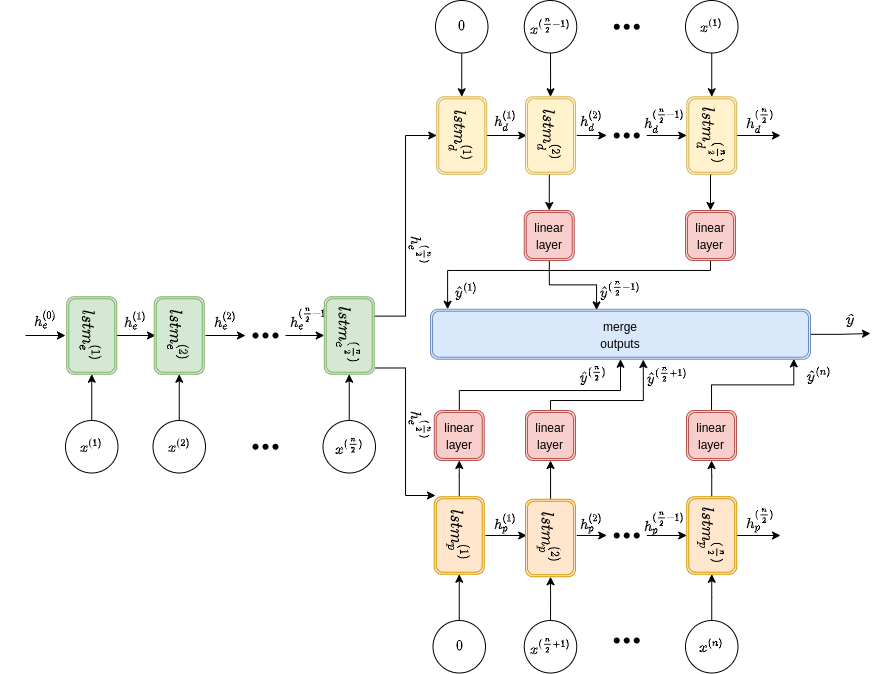
\includegraphics[width=1.0\textwidth]{img/composite_model.png}
	\caption{Composite model for input reconstruction and future prediction}
	\label{fig:experiments:unsupervised_lstm_composite}
\end{figure}	

\section{Self-supervised Pre-training for Transformer Networks} \label{sec:experiments:transformer}

Like with the \gls{lstm} we devised a series of proxy tasks for pre-training the model in self-supervised fashion. Since the information flow is different in transformer models than it is in \glspl{lstm}, the pre-training task \textit{Predict Packets} \ref{sec:experiments_lstm} we used for the \gls{lstm} is no longer feasible. While the \gls{lstm} at each stage only has access to all the tokens it processed up to this point, the transformer has access to all input tokens at each stage of the execution which is one of the benefits of self-attention \cite{attention}. Contrary to our expectations, supervised training with 90\% of the dataset on the transformer takes longer to converge than on the \gls{lstm} in terms of real time. In other words, when training the \gls{lstm} and the transformer network with the same amount of data for the same amount of time, the \gls{lstm} produces better results. In the following sections we describe the pre-training methods we used to pre-train the transformer network.

\begin{table}[H]
	\scalebox{0.8}{
	\begin{tabular}{cccccccc}
		\textbf{\#} & \textbf{Dataset} & \textbf{Subset} & \textbf{Training} \% & \textbf{Training Eps.} & \textbf{Proxy Task} & \textbf{Pretr.} \% & \textbf{Pretr. Eps.} \\ \hline
		3.1.1 & CIC-IDS2017 & -          & 10          & 50            & NONE       & 0         & 0           \\
		3.1.2 & CIC-IDS2017 & -          & 10          & 50            & AUTO       & 80        & 10          \\
		3.1.3 & CIC-IDS2017 & -          & 10          & 50            & OBSCURE      & 80        & 10          \\
		3.1.4 & CIC-IDS2017 & -          & 10          & 50            & MASK      & 80        & 10          \\
		3.2.1 & CIC-IDS2017 & -          & 1           & 200           & NONE       & 0         & 0           \\
		3.2.2 & CIC-IDS2017 & -          & 1           & 200           & AUTO       & 80        & 10          \\
		3.2.3 & CIC-IDS2017 & -          & 1           & 200           & OBSCURE      & 80        & 10          \\
		3.2.4 & CIC-IDS2017 & -          & 1           & 200           & MASK      & 80        & 10          \\
		3.3.1 & CIC-IDS2017 & CIC17\_10  & -           & 600           & NONE       & 0         & 0           \\
		3.3.2 & CIC-IDS2017 & CIC17\_10  & -           & 600           & AUTO       & 80        & 10          \\
		3.3.3 & CIC-IDS2017 & CIC17\_10  & -           & 600           & OBSCURE      & 80        & 10          \\
		3.3.4 & CIC-IDS2017 & CIC17\_10  & -           & 600           & MASK      & 80        & 10          \\
		3.4.1 & UNSW-NB15    & -          & 10          & 50            & NONE       & 0         & 0           \\
		3.4.2 & UNSW-NB15    & -          & 10          & 50            & AUTO       & 80        & 10          \\
		3.4.3 & UNSW-NB15    & -          & 10          & 50            & OBSCURE      & 80        & 10          \\
		3.4.4 & UNSW-NB15    & -          & 10          & 50            & MASK      & 80        & 10          \\
		3.5.1 & UNSW-NB15    & -          & 1           & 200           & NONE       & 0         & 0           \\
		3.5.2 & UNSW-NB15    & -          & 1           & 200           & AUTO       & 80        & 10          \\
		3.5.3 & UNSW-NB15    & -          & 1           & 200           & OBSCURE      & 80        & 10          \\
		3.5.4 & UNSW-NB15    & -          & 1           & 200           & MASK      & 80        & 10          \\
		3.6.1 & UNSW-NB15    & UNSW15\_10 & -           & 600           & NONE       & 0         & 0           \\
		3.6.2 & UNSW-NB15    & UNSW15\_10 & -           & 600           & AUTO       & 80        & 10          \\
		3.6.3 & UNSW-NB15    & UNSW15\_10 & -           & 600           & OBSCURE      & 80        & 10          \\
		3.6.4 & UNSW-NB15    & UNSW15\_10 & -           & 600           & MASK      & 80        & 10         
	\end{tabular}}
	\caption{Training and pre-training configurations for transformer model with different proxy tasks.}
	\label{table:experiments:transformer:configurations}
\end{table}

To make the effect of pre-training on the transformer more salient we tried different approaches like using two consecutive transformer encoder models in serial configuration. Only the first transformer model is pre-trained and for supervised fine-tuning it feeds its output, which hopefully constitutes an abstraction of the data, into the second model which is then trained with labeled data.
Another approach was to reset the deeper layers of the transformer model, as an abstract data representation might have formed in the earlier layers. The later layers might have been used to solve the proxy task based on this representation which are not needed and even disadvantageous for classification. We also tried tweaking the dropout rate, the number of attentions heads and the number of layers to improve performance. None of these methods achieved consistent improvements in our case.


\subsection{Obscure Features (OBSCURE)} \label{sec:experiments:transformer:mask_feature}

Analogous to the \textit{Mask Features} proxy task for the \gls{lstm}, we used the same method for pre-training the transformer.

\subsection{Auto Encoder (AUTO)} \label{sec:experiments:transformer:auto_encoder}

Auto encoder are an established concept when it comes to self-supervised learning \ref{sec:background:auto_encoder}. With this method input and target data are the same and the network is tasked with reconstructing the input data at the output. To prevent the network from simply "transporting" the input tokens through the network without having to learn anything, a form of regularization is introduced to force the network into learning an abstract representation of the data \cite{autoencoders}. In our case, we used a dropout rate of 20\% to introduce artificial noise into the input data. 

\subsection{Mask Packet (MASK)} \label{sec:experiments:transformer:mask_packet}

Same as with for the \gls{lstm}, one packet token is replaced with a mask vector $x_{mask} = [-1, ..., -1]^T$ containing $-1$ for each feature. The model is then tasked with reconstructing the omitted input. While for our \gls{lstm} model we found that this proxy task performs better if we also include the non-masked tokens into the loss calculation, here we calculate the loss only based on the difference between the masked token and the predicted token. For the \gls{lstm}, this task is very similar to the PREDICT task in section \ref{sec:experiments:lstm:predict_packet} with the difference that it is to predict only one token instead of every subsequent token. The transformer however is able to also take "future" packets, i.e. later packet tokens in the input sequence into account.
Since a packet in a flow can be seen as a word in a sentence, and the feature representation of a packet is similar to an embedded word vector, this pre-training task is analogous to the method used in \gls{bert} \cite{bert}. 

\newpage
